\documentclass[a0paper,landscape,final]{baposter}

\usepackage{times}
\usepackage{calc}
\usepackage{graphicx}
\usepackage{amsmath}
\usepackage{amssymb}
\usepackage{relsize}
\usepackage{multirow}
\usepackage{bm}
\usepackage{algorithm}
\usepackage{algorithmic}
\usepackage{subfigure}
\usepackage{slashbox}

\usepackage{graphicx}
\usepackage{multicol}

\usepackage{pgfbaselayers}
\pgfdeclarelayer{background}
\pgfdeclarelayer{foreground}
\pgfsetlayers{background,main,foreground}

\usepackage{helvet}
%\usepackage{bookman}
\usepackage{palatino}

\usepackage{enumitem}


\newcommand{\captionfont}{\footnotesize}

%\selectcolormodel{cmyk}

\graphicspath{{fig/}}

%%%%%%%%%%%%%%%%%%%%%%%%%%%%%%%%%%%%%%%%%%%%%%%%%%%%%%%%%%%%%%%%%%%%%%%%%%%%%%%%
%%%% Some math symbols used in the text
%%%%%%%%%%%%%%%%%%%%%%%%%%%%%%%%%%%%%%%%%%%%%%%%%%%%%%%%%%%%%%%%%%%%%%%%%%%%%%%%
% Format
\newcommand{\Matrix}[1]{\begin{bmatrix} #1 \end{bmatrix}}
\newcommand{\Vector}[1]{\Matrix{#1}}
\newcommand*{\SET}[1]  {\ensuremath{\mathcal{#1}}}
\newcommand*{\MAT}[1]  {\ensuremath{\mathbf{#1}}}
\newcommand*{\VEC}[1]  {\ensuremath{\bm{#1}}}
\newcommand*{\CONST}[1]{\ensuremath{\mathit{#1}}}
\newcommand*{\norm}[1]{\mathopen\| #1 \mathclose\|}% use instead of $\|x\|$
\newcommand*{\abs}[1]{\mathopen| #1 \mathclose|}% use instead of $\|x\|$
\newcommand*{\absLR}[1]{\left| #1 \right|}% use instead of $\|x\|$

\def\norm#1{\mathopen\| #1 \mathclose\|}% use instead of $\|x\|$
\newcommand{\normLR}[1]{\left\| #1 \right\|}% use instead of $\|x\|$

%%%%%%%%%%%%%%%%%%%%%%%%%%%%%%%%%%%%%%%%%%%%%%%%%%%%%%%%%%%%%%%%%%%%%%%%%%%%%%%%
% Multicol Settings
%%%%%%%%%%%%%%%%%%%%%%%%%%%%%%%%%%%%%%%%%%%%%%%%%%%%%%%%%%%%%%%%%%%%%%%%%%%%%%%%
\setlength{\columnsep}{0.7em}
\setlength{\columnseprule}{0mm}


%%%%%%%%%%%%%%%%%%%%%%%%%%%%%%%%%%%%%%%%%%%%%%%%%%%%%%%%%%%%%%%%%%%%%%%%%%%%%%%%
% Save space in lists. Use this after the opening of the list
%%%%%%%%%%%%%%%%%%%%%%%%%%%%%%%%%%%%%%%%%%%%%%%%%%%%%%%%%%%%%%%%%%%%%%%%%%%%%%%%
\newcommand{\compresslist}{%
\setlength{\itemsep}{1pt}%
\setlength{\parskip}{0pt}%
\setlength{\parsep}{0pt}%
}


%%%%%%%%%%%%%%%%%%%%%%%%%%%%%%%%%%%%%%%%%%%%%%%%%%%%%%%%%%%%%%%%%%%%%%%%%%%%%%
%%% Begin of Document
%%%%%%%%%%%%%%%%%%%%%%%%%%%%%%%%%%%%%%%%%%%%%%%%%%%%%%%%%%%%%%%%%%%%%%%%%%%%%%

\begin{document}

%%%%%%%%%%%%%%%%%%%%%%%%%%%%%%%%%%%%%%%%%%%%%%%%%%%%%%%%%%%%%%%%%%%%%%%%%%%%%%
%%% Here starts the poster
%%%---------------------------------------------------------------------------
%%% Format it to your taste with the options
%%%%%%%%%%%%%%%%%%%%%%%%%%%%%%%%%%%%%%%%%%%%%%%%%%%%%%%%%%%%%%%%%%%%%%%%%%%%%%
\typeout{Poster Starts}
\background{
  \begin{tikzpicture}[remember picture,overlay]%
   \draw (current page.north west)+(-2em,-0em) node[anchor=north west] {\hspace{-2em}\includegraphics[height=1.1\textheight]{silhouettes_background}};
 \end{tikzpicture}%
}
\definecolor{blue}{RGB}{150,200,242}
\definecolor{darkblue}{RGB}{68,92,170}
\definecolor{brown}{RGB}{245,236,215}

\begin{poster}{
  % Show grid to help with alignment
  grid=false,
  % Column spacing
  colspacing=1em,
  % Color style
  %headerColorOne=cyan!20!white!90!black,
  %borderColor=cyan!30!white!90!black,
  %bgColorOne=cyan!10!white,
  headerColorOne=blue,
  borderColor=darkblue,
  bgColorOne=brown,
  boxColorOne=white,
  %bgColorOne=lighteryellow,
  %bgColorTwo=lightestyellow,
  %borderColor=reddishyellow,
  %headerColorOne=yellow,
  %headerColorTwo=reddishyellow,
  %headerFontColor=black,
  %boxColorOne=lightyellow,
  %boxColorTwo=lighteryellow,
  % Format of textbox
  textborder=roundedleft,
  % Format of text header
  eyecatcher=true,
  headerborder=open,
  headerheight=0.08\textheight,
  headershape=roundedright,
  headershade=plain,
  headerfont=\Large\textsf, %Sans Serif
  boxshade=plain,
%  background=shade-tb,
  background=plain,
  linewidth=2pt,
  columns=3
  }
  % Eye Catcher
  {{\begin{minipage}{1.5cm}
    \vspace{0.5cm}
	
\includegraphics[width=3cm]{ethzlogo_short} \\
    
\includegraphics[width = 3.35cm]{usclogo2.pdf}
\end{minipage}}
  } % No eye catcher for this poster. If an eye catcher is present, the title is centered between eye-catcher and logo.
  % Title
  {\sf %Sans Serif
  %\bf% Serif
  {\huge Estimating the 3D Layout of Indoor Scenes and its Clutter from Depth Sensors}}
  % Authors
  {\sf %Sans Serif
  % Serif
  Jian Zhang${}^1$\hspace{1cm}
  Kan Chen${}^2$\hspace{1cm}
  Alexander G. Schwing${}^1$\hspace{1cm}
  Raquel Urtasun${}^3$\\
  {\small ${}^1$ETH Zurich\hspace{1cm}${}^2$USC\hspace{1cm}${}^3$TTI Chicago}
  }
%  {{\begin{minipage}{1.5cm}	
\includegraphics[width=2.5cm]{fig/usclogo.pdf}
%    \end{minipage}}
%  }
  % University logo
  {{\begin{minipage}{1.5cm}
    \hfill
    
\includegraphics[width=1.5cm]{tticlogo.pdf}
  \end{minipage}}
  }

  \tikzstyle{light shaded}=[top color=baposterBGtwo!30!white,bottom color=baposterBGone!30!white,shading=axis,shading angle=30]

  % Width of left inset image
     \newlength{\leftimgwidth}
     \setlength{\leftimgwidth}{0.78em+8.0em}

%%%%%%%%%%%%%%%%%%%%%%%%%%%%%%%%%%%%%%%%%%%%%%%%%%%%%%%%%%%%%%%%%%%%%%%%%%%%%%
%%% Now define the boxes that make up the poster
%%%---------------------------------------------------------------------------
%%% Each box has a name and can be placed absolutely or relatively.
%%% The only inconvenience is that you can only specify a relative position
%%% towards an already declared box. So if you have a box attached to the
%%% bottom, one to the top and a third one which should be in between, you
%%% have to specify the top and bottom boxes before you specify the middle
%%% box.
%%%%%%%%%%%%%%%%%%%%%%%%%%%%%%%%%%%%%%%%%%%%%%%%%%%%%%%%%%%%%%%%%%%%%%%%%%%%%%
    %
    % A coloured circle useful as a bullet with an adjustably strong filling
    \newcommand{\colouredcircle}[1]{%
      \tikz{\useasboundingbox (-0.2em,-0.32em) rectangle(0.2em,0.32em); \draw[draw=black,fill=baposterBGone!80!black!#1!white,line width=0.03em] (0,0) circle(0.18em);}}

%%%%%%%%%%%%%%%%%%%%%%%%%%%%%%%%%%%%%%%%%%%%%%%%%%%%%%%%%%%%%%%%%%%%%%%%%%%%%%
  \headerbox{Overview}{name=overview,column=0,row=0}{
%%%%%%%%%%%%%%%%%%%%%%%%%%%%%%%%%%%%%%%%%%%%%%%%%%%%%%%%%%%%%%%%%%%%%%%%%%%%%%
{\bf Goal}

Boost layout estimation and clutter labeling with RGBD data

\vspace{0.07cm}
{\bf Motivation}
\vspace{-0.2cm}
\begin{itemize}[leftmargin=*]\compresslist
    %\setlength{\itemindent}{-1em}
	\item[-] Indoor layout estimation and clutter labeling are correlated
	\item[-] Kinect provides more reliable 2.5D cues for scene understanding
\end{itemize}

\vspace{-0.17cm}
{\bf Approach}

Jointly estimate layout and segment clutter and bounding faces

\vspace{-0.3cm}
\begin{center}
    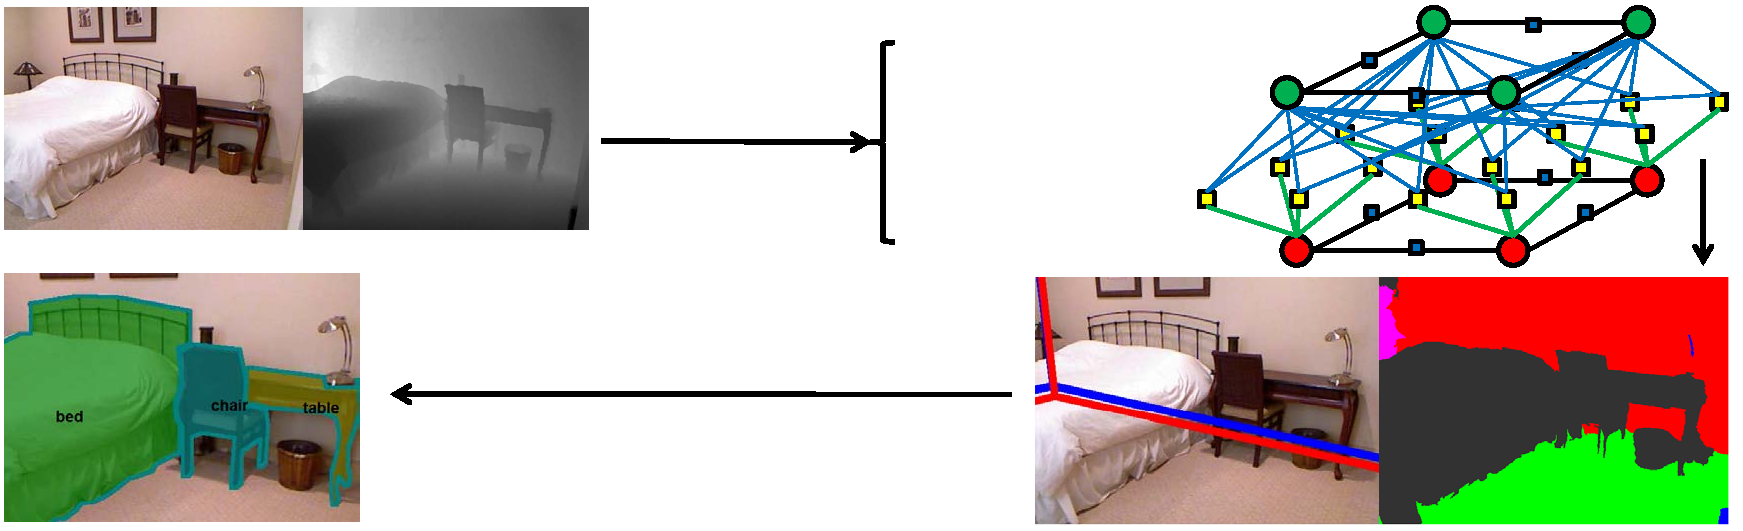
\includegraphics[width = 10.6cm]{../fig/Additional/overview_figure1.pdf}
    \put(-198,71){\bf \footnotesize Higher order}
    \put(-192,60){\bf \footnotesize modeling}
%    \put(-219,52){\bf \footnotesize Joint inference}
    \put(-195,27){\bf \footnotesize Finer-grain}
    \put(-206,16){\bf \footnotesize clutter semantics}
    \put(-146,81){\bf \footnotesize Layout}
    \put(-146,64){\bf \footnotesize Compatibility}
    \put(-146,47){\bf \footnotesize Segmentation}
    %\put{-205,85}{\bf \footnotesize Layout}
    %\put{-205, 85}{\bf \footnotesize Layout}
\end{center}

}
%%%%%%%%%%%%%%%%%%%%%%%%%%%%%%%%%%%%%%%%%%%%%%%%%%%%%%%%%%%%%%%%%%%%%%%%%%%%%%
  \headerbox{Model}{name=model,column=0,below=overview,above=bottom}{
%%%%%%%%%%%%%%%%%%%%%%%%%%%%%%%%%%%%%%%%%%%%%%%%%%%%%%%%%%%%%%%%%%%%%%%%%%%%%%
{\bf Overall model}
\begin{itemize}[leftmargin=*]\compresslist
    \vspace{-0.25cm}
    \item[-] Let $\bm{x}$ be clutter labeling and $\bm{y}$ the layout
    \item[-] Joint inference on layout, clutter labeling and compatibility with \\
        \vspace{-0.6cm}
        \begin{center}$\min_{\bm{x},\bm{y}}E_{layout}(\bm{y}) +  E_{labeling}(\bm{x}) + E_{comp}(\bm{x},\bm{y})$
        \end{center}
\end{itemize}
\vspace{-0.2cm}
{\bf Layout modeling}
\begin{itemize}[leftmargin=0pt]\compresslist
    %\setlength{\itemindent}{-1em}
    \vspace{-0.15cm}
	\item[] \emph{Parameterization:}
    \begin{itemize}[leftmargin=*]\compresslist
    %\setlength{\itemindent}{-1em}
    %\setlength{\itemindent}{-2.5em}
    %\item[-] 4 ray state variables $y_i \in {\cal Y}$, $i\in\{1,\ldots,4\}$
    %    \item[-] Horizontal ray $\bm{r}_1$, $\bm{r}_2$ from  $\operatorname{vp}_0$.  Vertical ray $\bm{r}_3$, $\bm{r}_4$ from $\operatorname{vp}_1$
    \item[-] $y_i$ are discretized states for the horizontal and vertical rays $\bm{r}_i$

	\item[-] Face $\alpha \in \mathcal{F} = \{\text{\emph{left-wall}, \emph{right-wall}, \emph{front-wall}, \emph{ceiling}, \emph{floor}}\}$

    \item[-] Front-wall is defined by 4 rays and other faces by 3 rays
    \end{itemize}
    \vspace{-0.37cm}
    \begin{center}
    \begin{tabular}{c c c}
        \includegraphics[width = .25\linewidth]{../Drawings/Parameterization.pdf}
        \put(-90,35){$\operatorname{vp}_0$}
		\put(-23,3){$\operatorname{vp}_1$}
		\put(-20,37){$\operatorname{vp}_2$}
		\put(-67,46){$y_1$}
		\put(-67,27){$y_2$}
		\put(-43,15){$y_3$}
		\put(-22,15){$y_4$}
		\put(0,48){$\bm r_1$}
		\put(0,25){$\bm r_2$}
		\put(-50,59){$\bm r_3$}
        \put(-20,59){$\bm r_4$}
        & \hspace{0.2cm} \includegraphics[width = .25\linewidth]{../Drawings/IntegralGeometryNew3.pdf} \put(-89,35){$\operatorname{vp}_0$}
		\put(-23,3){$\operatorname{vp}_1$}
		\put(-22,37){$\operatorname{vp}_2$}
		\put(-67,46){$y_1$}
		\put(-67,27){$y_2$}
		\put(-43,15){$y_3$}
		%\put(-22,15){$y_4$}
		\put(0,48){$\bm r_1$}
		\put(0,25){$\bm r_2$}
		\put(-50,59){$\bm r_3$}
        %\put(-20,59){$\bm r_4$}
         & \hspace{0.3cm} \includegraphics[width = 2.7cm]{../fig/SuperpixelVisuals/spixel_216.pdf}
        %\\ (a) & (b) & (c)
    \end{tabular}
    \end{center}
    \vspace{-0.5cm}
    \item[] \emph{Energy of layout:}
    \vspace{-0.1cm}
    \begin{itemize}[leftmargin=*]\compresslist
    %\setlength{\itemindent}{-1em}
    \item[-] Utilize Geometric Context (GC) and Orientation Map (OM) as cues
    \item[-] $\phi_{lay,\alpha}(\bm{y})$ is the sum of image cues in face $\alpha$. The layout energy is
        \vspace{-0.05cm}
        \begin{center}$E_{layout}(\bm{y}) = \sum_{\alpha\in\mathcal{F}} w_{lay,\alpha}^\top \phi_{lay,\alpha}(\bm{y}) $
         \end{center}

        \item[-] High order energy decomposed to pairwise [Schwing et al., 2012] (See middle figure)
            \vspace{-0.1cm}
            \begin{center}
            $\phi_{lay, \text{\emph{ left-wall}}}(y_1, y_2, y_3) = \phi_{lay, \text{\emph{green}}}(y_1, y_3) - \phi_{lay, \text{\emph{blue}}}(y_2, y_3)$
            \end{center}
            \vspace{-0.075cm}
        %E.g. left wall (in the right figure) is the green region subtracting the blue one.
    \end{itemize}
\end{itemize}

\vspace{-0.1cm}
{\bf Clutter labeling}
\begin{itemize}[leftmargin=*] \compresslist
    \vspace{-0.1cm}
    \item[-] We extend LAB SLIC superpixel with depth gradient information
    \item[-] Variable $x_i\in \mathcal{L} = \mathcal{F} \cup \{\text{\emph{clutter}}\}$

%\end{itemize}
%\vspace{-0.1cm}
%\vspace{-0.2cm}
%\begin{itemize}[leftmargin=*]\compresslist
    %\setlength{\itemindent}{-1em}
    \item[-] GC, OM, superpixel centroid and normal as unary cues
    \item[-] Binary physical relation (e.g. floor is below clutter) as pairwise cues
\end{itemize}

%\vspace{2cm}
%\begin{minipage}{6.7cm}
%{\bf Branch-and-Bound for exact inference:}
%
%%\vspace{-0.6cm}
%%\begin{center}
%%\line(1,0){190}
%%\end{center}
%%
%%\vspace{-0.5cm}
%%{\bf Algorithm:} Branch-and-Bound inference
%
%\begin{center}
%\line(1,0){190}
%\end{center}
%
%%\begin{center}
%%\begin{algorithmic}
%%\STATE put pair $(\bar{f}({\cal Y}),{\cal Y})$ into queue, set $\hat {\cal Y} = {\cal Y}$
%%\REPEAT
%%\STATE split $\hat {\cal Y} = \hat {\cal Y}_1 \times \hat {\cal Y}_2$ with $\hat {\cal Y}_1\cap\hat {\cal Y}_2 = \emptyset$
%%\STATE put pair $(\bar{f}(\hat{\cal Y}_1),\hat{\cal Y}_1)$ into queue
%%\STATE put pair $(\bar{f}(\hat{\cal Y}_2),\hat{\cal Y}_2)$ into queue
%%\STATE retrieve $\hat {\cal Y}$ having highest score
%%\UNTIL{$|\hat {\cal Y}| = 1$}
%%\end{algorithmic}
%%\end{center}
%
%\begin{center}
%\line(1,0){190}
%\end{center}
%
%{\bf Requirements:} Definition of
%\begin{enumerate}\compresslist
%\item Sets of hypothesis
%\item Interval scoring function $\bar{f}$
%\item Tight but efficiently computable bounds
%\end{enumerate}
%\end{minipage}
%\hspace{0.5cm}
%\vspace{0.3cm}
%{\bf Difficulty:} How to design an efficient yet exact inference algorithm?
  }
%%%%%%%%%%%%%%%%%%%%%%%%%%%%%%%%%%%%%%%%%%%%%%%%%%%%%%%%%%%%%%%%%%%%%%%%%%%%%%
  \headerbox{Model}{name=modelcont,column=1,row=0}{
%%%%%%%%%%%%%%%%%%%%%%%%%%%%%%%%%%%%%%%%%%%%%%%%%%%%%%%%%%%%%%%%%%%%%%%%%%%%%%
\emph{Energy of labeling:}
\vspace{-0.2cm}
\begin{itemize}[leftmargin=*]\compresslist
    \setlength{\itemindent}{-0.38em}
    \item[-] $\!\!\!E_{labeling}(\bm{x})\!\! =\!\!\!\!\sum\limits_{\beta\in\mathcal{L}}\sum\limits_{i = 1}^n \!\!w_{lab,\beta}^\top \phi_{lab,\beta,i}(x_i) + \!\!\!\!\!
            \sum\limits_{\beta,\gamma\in\mathcal{L}}\sum\limits_{(i,j)\in E} \!\!\!\!\!\!w_{lab,\beta,\gamma}^\top \phi_{lab,\beta,\gamma,i,j}(x_i,x_j)$
\end{itemize}
\vspace{-0.1cm}
{\bf Compatibility modeling}
\begin{itemize}[leftmargin=*, align = left]\compresslist
    \setlength{\itemindent}{-1em}
    \vspace{-0.20cm}
    \begin{minipage}{5.3cm}
    \vspace{-0.45cm}
    \item[] \emph{Idea:}
    \vspace{-0.1cm}
    \begin{itemize}[leftmargin=0pt, align = left]\compresslist
    %\setlength{\itemindent}{1em}
        \item[-] {Pixel-wise consistent estimation of bounding faces from layout estimation and clutter labeling}
    \end{itemize}
    \end{minipage}
    \hspace{0.25cm}
    \vspace{-0.05cm}
    \begin{minipage}{5cm}
        \includegraphics[width = .79\linewidth] {../Drawings/ParameterizationCompatibility.pdf}
        \put(-115,65){$\operatorname{vp}_0$}
		\put(-40,5){$\operatorname{vp}_1$}
		\put(-45,63){$\operatorname{vp}_2$}
		\put(-97,68){$y_1$}
		\put(-97,48){$y_2$}
		\put(-65,15){$y_3$}
		%\put(-30,15){$y_4$}
		\put(2,75){$\bm r_1$}
		\put(2,38){$\bm r_2$}
		\put(-72,90){$\bm r_3$}
        %\put(-25,75){$\bm r_4$}
        %\\{\huge (a) & (b)}
    \end{minipage}
    \vspace{-0.6cm}
    \item[] \emph{Energy of compatibility:}
    \vspace{-0.15cm}
    \begin{itemize}[leftmargin = 0pt]\compresslist
        \item[-] $\bm{p}$ is an arbitrary pixel in a superpixel labeled as class $x(\bm{p}) \in \mathcal{L}$
        \item[-] Accumulate overlapping of face $\alpha\!\in\!\mathcal{F}$ from layout and class $\beta\!\in\!\mathcal{L}$ from clutter labeling. $\gamma(\bm{y},\alpha)$ is the face $\alpha$ in layout $\bm{y}$. \\
            \vspace{-0.55cm}
            \begin{center}
                $\phi_{comp,\alpha,\beta}(\bm{x},\bm{y}) = \sum_{\bm{p} \in \gamma(\bm{y},\alpha)} \delta(x(\bm{p}) = \beta)$
            \end{center}
        \vspace{-0.1cm}
        \item[-] Sum over all the  $(\alpha, \beta)$ pair, we get third order terms
        \vspace{-0.1cm}
        \begin{center}
        $E_{comp}(\bm{x},\bm{y}) = \sum_{\alpha\in\mathcal{F}} \sum_{\beta\in\mathcal{L}} w_{comp,\alpha,\beta} \phi_{comp,\alpha,\beta}(\bm{x},\bm{y})$
        \end{center}
        \vspace{-0.15cm}
    \end{itemize}
\end{itemize}

%
%
%{\bf 1. Hypothesis space:} Product space $\hat{\cal Y} = \prod_{i=1}^4 Y_i$ with
%
%\begin{equation*}
%Y_i = [y_i^{\operatorname{min}}, y_i^{\operatorname{max}}]
%\end{equation*}
%
%{\bf 2. Interval scoring function:}
%
%Properties of interval function
%\begin{enumerate}\compresslist
%	\item Upper bound to the true cost: $\forall \bm y\in \hat{\cal Y}$, $\bar{f}(\hat{\cal Y}) \geq \bm w^\top\phi(\bm x,\bm y)$
%	\item Exactness for single hypothesis: $\forall \bm y\in {\cal Y}$, $\bar{f}(\bm y) = \bm w^\top\phi(\bm x,\bm y)$
%\end{enumerate}
%
%Let $\bm w^\top\phi(\bm x,\bm y) = \sum_{\alpha\in{\cal F}} \left(f_\alpha^{+}(\bm x,\bm y) + f_\alpha^{-}(\bm x,\bm y)\right)$ with
%\begin{eqnarray*}
%f_\alpha^{+}(\bm x,\bm y) &=& \sum_{\{(i,r) : i\in\{o,g\},w_{i,\alpha,r}>0\}} \!\!\!\!\!\!\!\!\!\!\!\!w_{i,\alpha,r}\phi_{i,\alpha,r}(\bm x,\bm y_\alpha), \\
%f_\alpha^{-}(\bm x,\bm y) &=& \sum_{\{(i,r) : i\in\{o,g\},w_{i,\alpha,r}\leq 0\}} \!\!\!\!\!\!\!\!\!\!\!\!w_{i,\alpha,r}\phi_{i,\alpha,r}(\bm x,\bm y_\alpha).
%\end{eqnarray*}
%
%{\bf Bound: Sum the maximal positive contribution of the considered interval and subtract the minimal negative part.}
%
%Example: $\bar{f}_{{\text{\emph{front-wall}}}}(\hat{\cal Y}) = f^{+}_{{\text{\emph{front-wall}}}}(\bm x,\bm y^{\operatorname{max}}) + f^{-}_{{\text{\emph{front-wall}}}}(\bm x,\bm y^{\operatorname{min}})$
%
%\vspace{0.2cm}
%{\bf 3. Efficient computation:} Integral Geometry (integral images in accordance with vanishing points) allows computation of bounds in constant time.
  }

%%%%%%%%%%%%%%%%%%%%%%%%%%%%%%%%%%%%%%%%%%%%%%%%%%%%%%%%%%%%%%%%%%%%%%%%%%%%%%%
  \headerbox{Alternating Inference}{name=infer,column=1,below=modelcont,span=1}{
%%%%%%%%%%%%%%%%%%%%%%%%%%%%%%%%%%%%%%%%%%%%%%%%%%%%%%%%%%%%%%%%%%%%%%%%%%%%%
\vspace{-0.4cm}
\begin{algorithm}[H]
\caption{Alternating Inference}
\begin{algorithmic}[1]
 \STATE ${\bm{y}}^{(0)} = \min_{\bm{y}} E_{layout}(\bm{y})$
\FORALL {$i = 1:M$}
    \STATE ${\bm{x}}^{(i)} = \min_{\bm{x}} E_{labeling}(\bm{x}) + E_{comp}(\bm{x},\bm{y}^{(i-1)})$
    \STATE ${\bm{y}}^{(i)} = \min_{\bm{y}} E_{layout}(\bm{y}) + E_{comp}(\bm{x}^{(i)},\bm{y})$
\ENDFOR
\STATE Return ${\bm{x}}^{(M)}, {\bm{y}}^{(M)}$
\end{algorithmic}
\label{alg:inf}
\end{algorithm}
\vspace{-0.7cm}
\begin{itemize}[leftmargin = *]\compresslist
    \item[-] Reduced to pairwise CRF in each iteration
    \item[-] Appealing results achievable with only 2 rounds of alternating
    \item[-] Alternating approximation is faster than convergency of direct BP
\end{itemize}
\vspace{-0.3cm}

}

%%%%%%%%%%%%%%%%%%%%%%%%%%%%%%%%%%%%%%%%%%%%%%%%%%%%%%%%%%%%%%%%%%%%%%%%%%%%%%
  \headerbox{Fast Integral Geometry}{name=IG,column=1,below=infer, above=bottom}{
%%%%%%%%%%%%%%%%%%%%%%%%%%%%%%%%%%%%%%%%%%%%%%%%%%%%%%%%%%%%%%%%%%%%%%%%%%%%%%
%{\bf Problem}
Complexity of naive Integral Geometry computation is $\bm{O(N^2R^2)}$. \\$N^2$ is the size of image and $R$ is the cardinality of each ray variable

\vspace{0.1cm}
\begin{minipage}{6cm}
{\bf $\bm{O(N^2)}$ solution}
\vspace{-0.25cm}
\begin{itemize}[leftmargin=*]\compresslist
    %\setlength{\itemindent}{-1em}
    \item[-] Neighboring pixels lie in the same or neighboring bins of the ray grid
    %\begin{minipage}{5.5cm}
    %\vspace{-0.3cm}
    \item[-] Compute Integral Geometry by
    \begin{enumerate}[leftmargin=*]\compresslist
        \item Assign pixles to $R\!\times\!R$ bin array
        \item Accumulate for bins with assigned pixels
        \item Do Integral Image on $R\!\times\!R$ matrix
    \end{enumerate}
    %\item[-] Complexity is reduced to $\bm{O(MN)}$
    \end{itemize}
    \end{minipage}
    \begin{minipage}{4cm}
        \begin{figure}[H]
        \vspace{-0.33cm}
        \centering
        \includegraphics[width=3.7cm]{../Drawings/ParameterizationFastCompNew2.pdf}
        \put(-106,43){$\operatorname{vp}_1$}
        \put(-17,4){$\operatorname{vp}_2$}
        %\put(-150,130){{\small$y_3 = 1$}}
        \put(-78,91){{\small$y_3 = 2$}}
        \put(-48,91){{\small$y_3 = 3$}}
        %\put(-60,130){{\small$y_3 = 4$}}
        %\put(-15,140){{\small$y_1 = 1$}}
        \put(-2,71){{\small$y_1 = 2$}}
        \put(-2,52){{\small$y_1 = 3$}}
        %\put(-15,65){{\small$y_1 = 4$}}
    \end{figure}
\end{minipage}


%
%
%{\bf Layout data set:}
%
%{\small
%\begin{center}
%\begin{tabular}{|c||c|c|c|c|c|}
%\hline
%&  OM & GC & OM + GC & Others & Time\\ \hline \hline
%[Hoiem07]  &- &28.9&-&-&- \\ \hline
%%\cite{Hedau09} (a) & - &26.5& -\\ \hline
%[Hedau09]  &-  &21.2 &-&-&-\\ \hline
%[Wang10]  & 22.2 &-&-&-&- \\ \hline
%[Lee10]  & 24.7 & 22.7 & 18.6&-&-\\ \hline
%%Ours (SVM$^{struct}$) & {\bf 20.0} & {\bf 18.8} & {\bf 17.3} \\ \hline
%%Ours (best struct-pred) & {\bf 18.38} & {\bf 15.22} & {\bf 13.86}\\ \hline
%%Ours (median struct-pred) & {\bf 18.38} & {\bf 15.22} & {\bf 13.86}\\ \hline
%%Ours (median struct-pred) & {\bf 19.4} & {\bf 16.2} & {\bf 14.7}\\ \hline		%CVPR no flip
%%Ours (SVM$^{\text{struct}}$) & {\bf 19.5} & {\bf 18.2} & {\bf 16.8} \\ \hline
%%Ours (median struct-pred) & {\bf 18.9} & {\bf 15.6} & {\bf 14.0}\\ \hline
%[Pero12] & - & - & - & 16.3 & 12min \\ \hline
%[Schwing12] & {\bf 18.64} & {\bf 15.35} & {\bf 13.59}&-& 0.15s \\ \hline
%Ours & {\bf 18.63} & {\bf 15.35} & {\bf 13.59}&-&{\bf 0.007s}\\ \hline
%\end{tabular}
%\end{center}
%}

  }


%%%%%%%%%%%%%%%%%%%%%%%%%%%%%%%%%%%%%%%%%%%%%%%%%%%%%%%%%%%%%%%%%%%%%%%%%%%%%%
  \headerbox{Results}{name=results,column=2,span=1,row=0}{
%%%%%%%%%%%%%%%%%%%%%%%%%%%%%%%%%%%%%%%%%%%%%%%%%%%%%%%%%%%%%%%%%%%%%%%%%%%%%%
{\bf Experiment setup}
\vspace{-0.2cm}
\begin{itemize}[leftmargin=*]\compresslist
    \item[-] 202 training and 101 testing samples from NYU depth V2 dataset
    \item[-] Inference with Convex Belief Propogation [Schwing et.al, 2011]
    \item[-] Training with structured SVM [Tsochantaridis et al., 2004]
    %\item[-] RGB features include Geometric Context and Orientation Map
%    \item[-] Layout features include Geometric Context, Orientation Map \\ Labeling Features include Geometric Context, 3D superpixel centroid and orientation, spatial relationship for superpixel pairs
\end{itemize}

\vspace{-0.15cm}
{\bf Comparison to the state-of-the-art}
\begin{table}[H]
\vspace{-0.3cm}
\centering
\begin{tabular}{|c||c|c|}
\hline
& layout error & labeling error\\ \hline
GC [Hoiem et al, 2007] &  -- & 26.38\% \\
\hline
[Schwing et al., 2012] & 13.66\% & -- \\ \hline
Ours rgb & 13.94\% & 23.68\% \\
\hline
Ours rgb depth& {\bf 8.04\%} & {\bf 13.65\%} \\
\hline
\end{tabular}
\end{table}

\vspace{-0.25cm}
{\bf Clutter labeling with finer-grain segmentation}
\vspace{-0.2cm}
\begin{itemize}[leftmargin=*]\compresslist
    \item[-] Six classes IOU of clutter labeling:\\
    \vspace{-0.6cm}
    \begin{table}[H]
        \centering
        {\footnotesize
        \begin{tabular}{|l||cccccc|c|}\hline
        IOU & ceiling & floor & left & front & right & clutter & average\\\hline
        rgb & 53.57 & 51.48 & 61.71 & 69.21 & 63.37 & 58.26 & 59.60\\
        rgb depth & {\bf 80.36} & {\bf 85.84} & {\bf 68.93} & {\bf 77.27} & {\bf 75.15} & {\bf 72.47} & {\bf 76.67}\\\hline
        \end{tabular}
        }
    \end{table}
    \vspace{-0.3cm}
    \item[-] We employ [Ren et al., 2012] to train classifiers for splitting clutter into 6 furniture classes. Clutter semantics classifier is trained with RGBD kernel descriptors: gradient, color, local binary pattern, depth gradient, surface normal and self-similarity
        \item[-] The IOU of finer-grain segmentation:
        \vspace{-0.3cm}
        \begin{table}[H]
        \centering
        \addtolength{\tabcolsep}{-2pt}
        {\small
        \begin{tabular}{|c||c|c|c|c|c|c|c|}
        \hline
         C in structSVM& 100        & 300        & 500        & 1000        & 3000        & 5000        & 10000\\
        \hline
        %\hline
        toilet &    35.67 &    35.72 &    37.19 &    36.03 &    39.54 &    38.30 &    32.02\\
        \hline
        bed &     43.69 &    43.59 &    43.42 &    43.46 &    43.00 &    43.47 &    42.49\\
        \hline
        table &   16.90 &    20.90 &    21.29 &    21.21 &    20.60 &    20.98 &    21.02\\
        \hline
        cabinet &    20.68 &    20.61 &    21.49 &    21.26 &    21.43 &    19.23 &    19.60\\
        \hline
        sofa &    32.50 &    32.28 &    32.90 &    32.88 &    32.86 &    32.64 &    32.11\\
        \hline
        chair &   35.89 &    35.90 &    36.18 &    36.13 &    35.96 &    35.00 &    35.05\\
        \hline
    \end{tabular}
    }
    \end{table}
\end{itemize}

\vspace{-0.25cm}
{\bf Speed improvement of Integral Geometry}

 The speed of 640$\times$480 Integral Geometry is reduced from $7s$ to $\bm{0.32s}$.

\vspace{0.1cm}
{\bf Qualitative results}
\vspace{-0.25cm}
\begin{figure}[H]
    \centering
    \includegraphics[width = \linewidth]{fig/Additional/qualitative_results10.pdf}
\end{figure}
\vspace{-0.27cm}
%{\bf Bedroom data set:}
%
%{\small
%\begin{center}
%\begin{tabular}{|c||c|c|c|c|c|}
%\hline
%& [Pero11] & [Hoiem07] & [Hedau09] & [Schwing12] & Ours \\ \hline
%Error [\%] & 29.59 & 23.04 & 22.94 & {\bf 16.46} & {\bf 16.46} \\ \hline
%Time [s] & - & - & - & 0.17 & {\bf 0.007} \\ \hline
%\end{tabular}
%\end{center}
%}
%
%{\bf Percentage of completed test set samples:} Layout data set
%
%{\bf Timing:}
%
%\begin{center}
%{\footnotesize
%\begin{tabular}{cc}
%Layout data set & Bedroom data set\\
%\begin{tabular}{|c||c|c|}\hline
% & SSVM & [Hazan10] \\ \hline \hline
%[Schwing12] & 0.449 s & 0.146 s \\\hline
%Ours & {\bf 0.011 s} & {\bf 0.007 s}\\\hline
%\end{tabular}
%&
%\begin{tabular}{|c||c|c|}\hline
% & SSVM & [Hazan10] \\ \hline \hline
%[Schwing12] & 0.576 s & 0.169 s \\\hline
%Ours & {\bf 0.010 s} & {\bf 0.007 s}\\\hline
%\end{tabular}
%\end{tabular}
%}
%\end{center}
%
%{\bf Iterations vs Error:}
%
%{\bf Success cases:}\vspace{0.1cm}
%
%
%{\bf Failure cases:}\vspace{0.1cm}


  }%
%%%%%%%%%%%%%%%%%%%%%%%%%%%%%%%%%%%%%%%%%%%%%%%%%%%%%%%%%%%%%%%%%%%%%%%%%%%%%%%
%  \headerbox{References}{name=references,column=2,below=results,above=bottom}{
%%%%%%%%%%%%%%%%%%%%%%%%%%%%%%%%%%%%%%%%%%%%%%%%%%%%%%%%%%%%%%%%%%%%%%%%%%%%%%%
%    \smaller
%    \vspace{-0.4em}
%    \bibliographystyle{ieee}
%    \renewcommand{\section}[2]{\vskip 0.05em}
%      \begin{thebibliography}{1}\itemsep=-0.01em
%      \setlength{\baselineskip}{0.4em}
%      \bibitem{Alex ECCV 12}
%        A.G.~Schwing, T.~Hazan, M. Pollefeys, R. Urtasun.
%        \newblock Efficeint Exact Inference for3D Indoor Scene Understanding
%        \newblock In {\em ECCV 2012}
%      \bibitem{Xiaofeng CVPR 2012}
%        X.~Ren, L.~Bo, D. Fox.
%        \newblock RGB-(D) Scene Labeling: Features and Algorithms.
%        \newblock In {\em CVPR 2012}
%      \end{thebibliography}
%
%%  \smaller
%%    \vspace{-0.4em}
%%    \bibliographystyle{ieee}
%%    \renewcommand{\section}[2]{\vskip 0.05em}
%%      \begin{thebibliography}{1}\itemsep=-0.01em
%%      \setlength{\baselineskip}{0.4em}
%%      \bibitem{Alex ECCV 12}
%%        A.G.~Schwing, T.~Hazan, M. Pollefeys, R. Urtasun.
%%        \newblock {O}ptimal {S}tep {N}onrigid {ICP} {A}lgorithms for {S}urface {R}egistration
%%        \newblock In {\em CVPR 2007}
%%      \bibitem{amberg08:recognition}
%%        B.~Amberg, R.~Knothe, T. Vetter.
%%        \newblock Expression Invariant Face Recognition with a 3D Morphable Model
%%        \newblock In {\em AFGR 2008}
%%      \end{thebibliography}
%
%
%  }%

\end{poster}%
%
\end{document}
